% Modern editorial, markup and figure/layout contributions: CC-BY-SA-4.0.
% Historical text and illustrations: Leonhard Euler (1744), public domain.
% Component scope and upstream attribution: see RIGHTS.md.
% Vector redrawing after E65, Tabula V. Schematic coordinates.
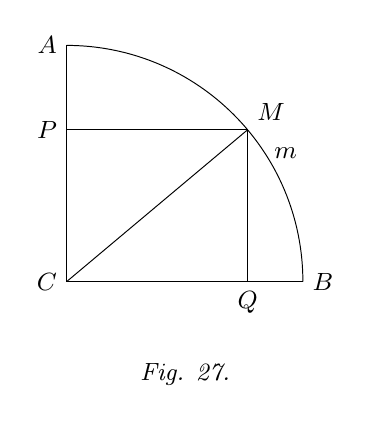
\begin{tikzpicture}[x=1cm,y=1cm,line width=.35pt,font=\small]
\draw (0,3)--(0,0)--(3,0);\draw (0,3) arc[start angle=90,end angle=0,radius=3];
\draw (0,1.92836)--(2.29813,1.92836)--(2.29813,0);\draw (0,0)--(2.29813,1.92836);
\node[left] at (0,3) {$A$};\node[left] at (0,0) {$C$};\node[right] at (3,0) {$B$};
\node[left] at (0,1.92836) {$P$};\node[below] at (2.29813,0) {$Q$};
\node[above right] at (2.29813,1.92836) {$M$};\node[right] at (2.516,1.634) {$m$};
\node[anchor=north] at ([yshift=-4mm]current bounding box.south) {\textit{Fig. 27.}};
\end{tikzpicture}
